\documentclass[11pt,a4paper]{article}
\usepackage[spanish,es-nodecimaldot]{babel}	% Utilizar español
\usepackage[utf8]{inputenc}					% Caracteres UTF-8
\usepackage{graphicx}						% Imagenes
\usepackage[hidelinks]{hyperref}			% Poner enlaces sin marcarlos en rojo
\usepackage{fancyhdr}						% Modificar encabezados y pies de pagina
\usepackage{float}							% Insertar figuras
\usepackage[textwidth=390pt]{geometry}		% Anchura de la pagina
\usepackage[nottoc]{tocbibind}				% Referencias (no incluir num pagina indice en Indice)
\usepackage{enumitem}						% Permitir enumerate con distintos simbolos
\usepackage[T1]{fontenc}					% Usar textsc en sections
\usepackage{amsmath}						% Símbolos matemáticos
\usepackage{subcaption}
\usepackage{caption}


\usepackage{listings}
\usepackage{xcolor}
 
\definecolor{codegreen}{rgb}{0,0.6,0}
\definecolor{codegray}{rgb}{0.5,0.5,0.5}
\definecolor{codepurple}{rgb}{0.58,0,0.82}
\definecolor{backcolour}{rgb}{0.95,0.95,0.92}
 
\lstdefinestyle{mystyle}{
    backgroundcolor=\color{backcolour},   
    commentstyle=\color{codegreen},
    keywordstyle=\color{magenta},
    numberstyle=\tiny\color{codegray},
    stringstyle=\color{codepurple},
    basicstyle=\ttfamily\footnotesize,
    breakatwhitespace=false,         
    breaklines=true,                 
    captionpos=b,                    
    keepspaces=true,                 
    numbers=left,                    
    numbersep=5pt,                  
    showspaces=false,                
    showstringspaces=false,
    showtabs=false,                  
    tabsize=4,
    language=Python
}
 
\lstset{style=mystyle}

% Comando para poner el nombre de la asignatura
\newcommand{\asignatura}{Visión por Computador}
\newcommand{\autor}{Vladislav Nikolov Vasilev}
\newcommand{\titulo}{Trabajo 1}
\newcommand{\subtitulo}{Filtrado y Detección de Regiones}

% Configuracion de encabezados y pies de pagina
\pagestyle{fancy}
\lhead{\autor{}}
\rhead{\asignatura{}}
\lfoot{Grado en Ingeniería Informática}
\cfoot{}
\rfoot{\thepage}
\renewcommand{\headrulewidth}{0.4pt}		% Linea cabeza de pagina
\renewcommand{\footrulewidth}{0.4pt}		% Linea pie de pagina

\begin{document}
\pagenumbering{gobble}

% Pagina de titulo
\begin{titlepage}

\begin{minipage}{\textwidth}

\centering

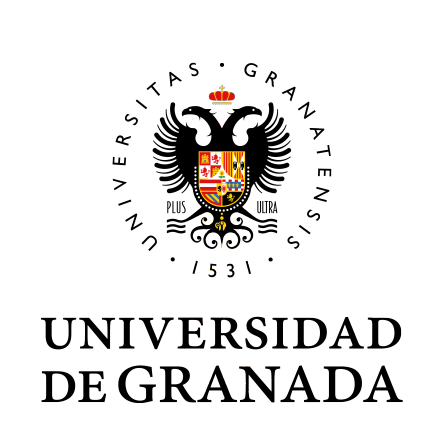
\includegraphics[scale=0.5]{img/ugr.png}\\

\textsc{\Large \asignatura{}\\[0.2cm]}
\textsc{GRADO EN INGENIERÍA INFORMÁTICA}\\[1cm]

\noindent\rule[-1ex]{\textwidth}{1pt}\\[1.5ex]
\textsc{{\Huge \titulo\\[0.5ex]}}
\textsc{{\Large \subtitulo\\}}
\noindent\rule[-1ex]{\textwidth}{2pt}\\[3.5ex]

\end{minipage}

\vspace{0.5cm}

\begin{minipage}{\textwidth}

\centering

\textbf{Autor}\\ {\autor{}}\\[2.5ex]
\textbf{Rama}\\ {Computación y Sistemas Inteligentes}\\[2.5ex]
\vspace{0.3cm}


\includegraphics[scale=0.3]{img/etsiit.jpeg}

\vspace{0.7cm}
\textsc{Escuela Técnica Superior de Ingenierías Informática y de Telecomunicación}\\
\vspace{1cm}
\textsc{Curso 2019-2020}
\end{minipage}
\end{titlepage}

\pagenumbering{arabic}
\tableofcontents
\thispagestyle{empty}				% No usar estilo en la pagina de indice

\newpage

\setlength{\parskip}{1em}

\section{\textsc{Ejercicio sobre filtros básicos}}

\noindent \textbf{USANDO LAS FUNCIONES DE OPENCV}: escribir funciones que implementen los siguientes puntos:

\begin{enumerate}[label=\textbf{\Alph*)}]
	\item \textbf{El cálculo de la convolución de una imagen con una máscara 2D. Usar una Gaussiana 2D (GaussianBlur)
	y máscaras 1D dadas por getDerivKernels). Mostrar ejemplos con distintos tamaños de máscara, valores de
	sigma y condiciones de contorno. Valorar los resultados.}
	\item \textbf{Usar la función Laplacian para el cálculo de la convolución 2D con una máscara normalizada de
	Laplaciana-de-Gaussiana de tamaño variable. Mostrar ejemplos de funcionamiento usando dos tipos de
	bordes y dos valores de sigma: 1 y 3.}
\end{enumerate}

\subsection{Apartado A}

Para realizar todas las pruebas, vamos a utilizar una imágen en blanco y negro. De esta forma, los resultados se podrán
ver de forma más clara. Se puede utilizar cualquiera de las imágenes que se han proporcionado, pero vamos a utilizar
la foto del gato. A continuación se puede ver la imágen en cuestión:

\begin{figure}[H]
\centering
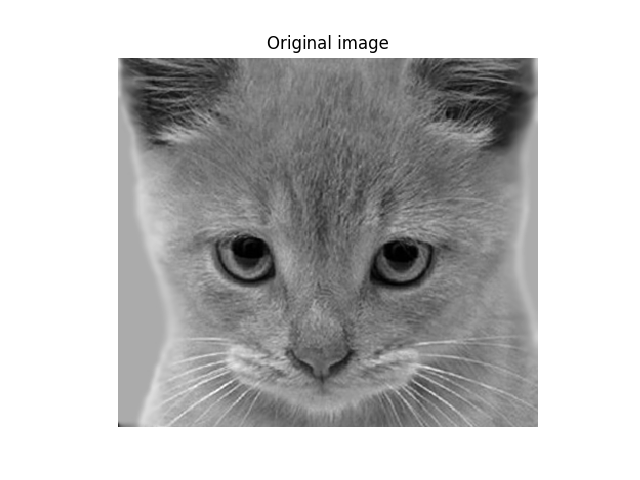
\includegraphics[scale=0.6]{img/cat.png}
\caption{Imágen original del gato en blanco y negro.}
\label{fig:cat}
\end{figure}

Antes de ver cuáles son los resultados y compararlos. Hace falta aclarar algunos puntos:

\begin{itemize}
	\item Cuando se cargan las imágenes, se convierten a \textit{float64}, para así tener más precisión a la hora de
	hacer las posteriores operaciones (aplicar filtros, sumar o restar imágenes, etc.), además de que así no nos limitamos
	a usar solo valores en el rango $[0, 255]$.
	\item Las operaciones para aplicar filtros de OpenCV aplican una correlación. Por tanto, para aplicar una convolución,
	se debe realizar un \textit{flip} del \textit{kernel}; esto es, darle la vuelta en el eje $X$ y en el eje $Y$.
	Como en todos los casos trabajaremos con \textit{kernels} separables, solo será necesario darles la vuelta en un sentido.
	\item Respecto al punto anterior, al trabajar con \textit{kernels} separables, con tal de mejorar la eficiencia,
	se puede aplicar primero el \textit{kernel} del eje $X$ y, sobre el resultado, aplicar el \textit{kernel} en el
	eje $Y$. Esto es mucho más rápido que aplicar directamente un \textit{kernel} 2D sobre la imágen, debido a que el
	número de operaciones es mucho menor.
\end{itemize}

Como en este ejercicio se piden aplicar \textit{kernels} de Gaussiana y de derivada, se han hecho funciones específicas
las cuáles pueden ser consultadas en el código. Estas funciones son \textit{gaussian\_kernel()} y \textit{derivative\_kernel()},
respectivamente. No se va a especificar exactamente lo que hacen debido a que solo obtienen los \textit{kernels} con los
parámetros adecuados (valores de $\sigma$ y tamaño de cada \textit{kernel} para el caso de la Gaussiana, y tamaño del
\textit{kernel} y número de veces que se deriva en cada eje en el caso de la derivada).

Lo que sí que es importante destacar es que estas dos funciones utilizan una común para realizar la convolución. Como se
dijo anteriormente, OpenCV realiza como tal la correlación, pero se puede aplicar una convolución realizando unos pocos cambios.
La función que se puede ver a continuación recibe un \textit{kernel} para cada eje y aplica el filtro mediante la
convolución:

\begin{lstlisting}[label={alg:apply-kernel}]
def apply_kernel(img, kx, ky, border):
    """
    Funcion que aplica un kernel separable sobre una imagen,
    realizando una convolucion

    Args:
        img: Imagen sobre la que aplicar el filtro
        kx: Kernel en el eje X
        ky: Kernel en el eje Y
        border: Tipo de borde
    Return:
        Devuelve una imagen filtrada
    """
    # Hacer el flip a los kernels para aplicarlos como una convolucion
    kx_flip = np.flip(kx)
    ky_flip = np.flip(ky)

    # Realizar la convolucion
    conv_x = cv.filter2D(img, cv.CV_64F, kx_flip.T,
    					 borderType=border)
    conv = cv.filter2D(conv_x, cv.CV_64F, ky_flip,
    				   borderType=border)

    return conv
\end{lstlisting}

Como se puede ver, se tiene que hacer un \textit{flip} de los \textit{kernels} para poder aplicar una convolución.
Al aplicar cada \textit{kernel} de forma separada mediante $filter2D$, se consigue una mayor eficiencia (como se ha
mencionado anteriormente). Es importante destacar que primero se aplica el \textit{kernel} sobre el eje de las $X$ y,
sobre el resultado obtenido, se aplica el \textit{kernel} en el eje $Y$. También es importante destacar que, cuando
se aplica el \textit{kernel} sobre el eje $X$, se le pasa la traspuesta del \textit{kernel}. Esto se debe a que
OpenCV proporciona los \textit{kernels} como vectores columnas, y para pasarlo por las filas, necesitamos que sea
un vector fila. Al traponer el vector columna obtenemos, como parece lógico, un vector columna.

Otra cosa muy importante a destacar son los \textit{kernels} que se van a utilizar. Uno de ellos es el \textit{kernel}
Gaussiano, el cuál es simétrico tanto en el eje $X$ como en el $Y$. Al aplicarlo, por tanto, se podría ahorrar la
operación del \textit{flip}, ya que lo va a dejar igual. Sin embargo, debido a que se ha implementado la función
para que sea genérica, se realiza esta operación. El otro \textit{kernel} que se utiliza es el de las derivadas,
que no es más que un \textit{kernel} de Sobel, el cuál combina alisamiento Gaussiano con la derivada.
A diferencia del anterior \textit{kernel}, este no es simétrico, y por tanto, la operación de
\textit{flip} no lo va a dejar igual; por tanto, no puede ser ahorrada en este caso.

Con esto comentado, ya podemos empezar a hablar de los resultados que se han obtenido. Para ello, vamos a comenzar
comentando los resultados que se obtienen para el filtro Gaussiano.

Lo primero que se ha probado es un \textit{kernel} de $5 \times 5$, variando los valores de $\sigma$ para ver cómo cambiaba.
A continuación se pueden ver los resultados:

\begin{figure}[H]
\begin{subfigure}{.5\textwidth}
	\centering
	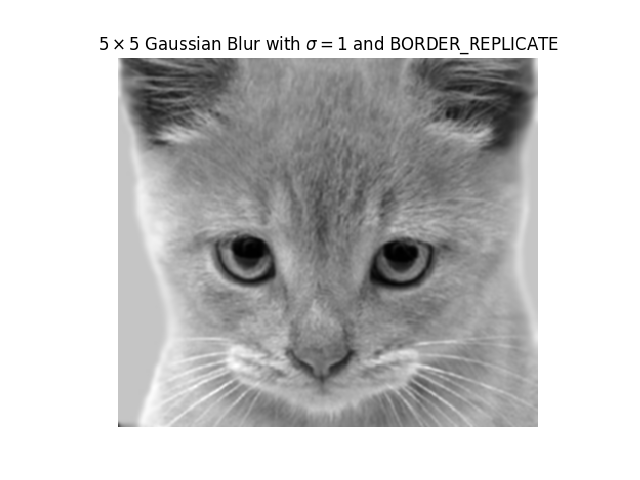
\includegraphics[scale=0.48]{img/gauss-sigma1.png}
	\subcaption{Filtro Gaussiano con $\sigma = 1$.}
	\label{fig:gauss-sigma1}
\end{subfigure}
\begin{subfigure}{.5\textwidth}
	\centering
	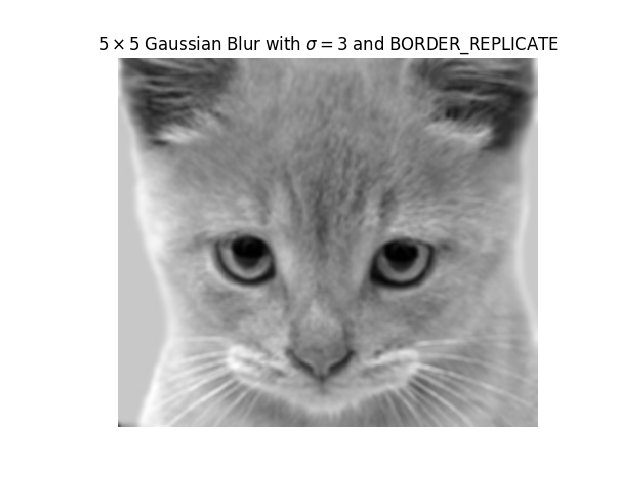
\includegraphics[scale=0.48]{img/gauss-sigma2.png}
	\subcaption{Filtro Gaussiano con $\sigma = 3$.}
	\label{fig:gauss-sigma2}
\end{subfigure}
\caption{Filtro Gaussiano con diferentes tamaños de $\sigma$.}
\label{fig:gauss-sigma}
\end{figure}

Como se puede ver, comparando cualquiera de las imágenes de la figura \ref{fig:gauss-sigma} con \ref{fig:cat}, existen ciertas
diferencias. Podemos ver claramente como al aplicar el filtro Gaussiano se ha perdido cierto detalle, ya que se están
eliminando las frecuencias altas. Además, si comparamos las figuras \ref{fig:gauss-sigma1} y \ref{fig:gauss-sigma2}, podemos
ver que a medida que aumentamos el tamaño de $\sigma$, se van perdiendo más detalles, ya que se emborrona más.

Se ha probado también a variar el tamaño de la máscara, conservando el mismo valor de $\sigma$, para ver qué es lo que sucede.
A continuación, se puede ver lo que se ha obtenido:

\begin{figure}[H]
\begin{subfigure}{.5\textwidth}
	\centering
	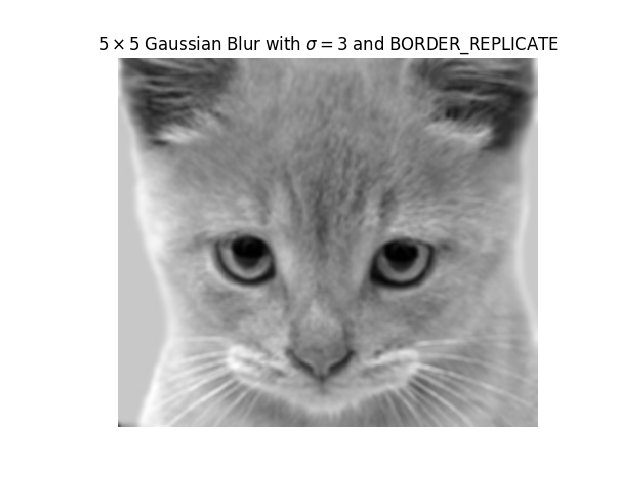
\includegraphics[scale=0.48]{img/gauss-sigma2.png}
	\subcaption{Filtro Gaussiano de tamaño $5 \times 5$.}
	\label{fig:gauss-sigma3}
\end{subfigure}
\begin{subfigure}{.5\textwidth}
	\centering
	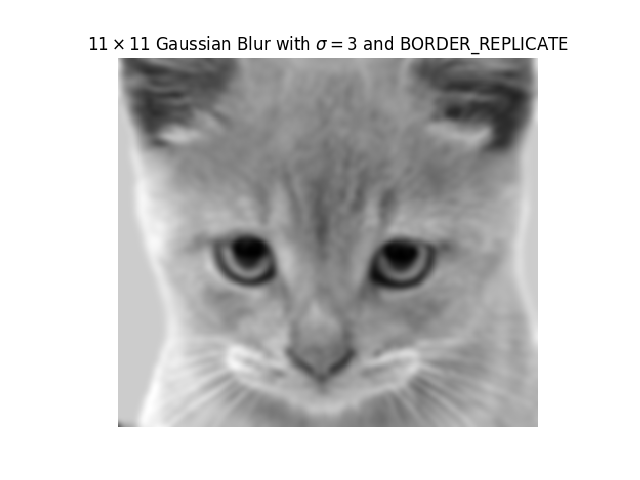
\includegraphics[scale=0.48]{img/gauss-size.png}
	\subcaption{Filtro Gaussiano de tamaño $11 \times 11$.}
	\label{fig:gauss-size1}
\end{subfigure}
\caption{Filtro Gaussiano con diferentes tamaños de \textit{kernel}.}
\label{fig:gauss-size}
\end{figure}

Tal y como se puede ver en la figura \ref{fig:gauss-size}, al modificar el tamaño del \textit{kernel} se han obtenido
diferentes resultados. Esto se debe a que más píxels forman parte de la máscara (como es obvio), y por tanto, se tiene
en cuenta una mayor parte de la Gaussiana. Por tanto, existe cierta dependencia entre esto dos valores (el tamaño del
\textit{kernel} y el valor de $\sigma$). A mayor $\sigma$, mayor tendrá que ser el tamaño de la máscara, para así poder
modelizar mejor el comportamiento de la función con los píxels vecinos. Si no se adaptase el tamaño del \textit{kernel},
se tendría que solo se coge una parte pequeña de la función Gaussiana más cercana al centro, ignorando el comportamiento
de los píxels más lejanos. Tampoco hay que coger un tamaño demasiado grande si el $\sigma$ es pequeño, ya que entonces
habrán muchos píxels que tendrán un valor muy próximo a 0 (aquellos que estén más alejados). En resumen, que hay
escoger de forma proporcional el tamaño del \textit{kernel} y el $\sigma$.

Para ver cómo afecta el tipo de borde a la imágen resultante, se han realizado una serie de pruebas variando el borde
utilizado a la hora de aplicar los \textit{kernels}. Para que los efectos fuesen notables, se ha tenido que escoger un
tamaño de máscara mucho más grande a los utilizados anteriormente. Esto se debe a que con una máscara pequeña no se
puede apreciar muy bien el resultado, debido a que no se coge mucha región fuera de los bordes de la imágen. El tamaño de
la máscara es de $101 \times 101$, permitiendo que se salga lo suficiente de la imágen para ver la influencia. A continuación
se pueden ver los resultados que se han obtenido:

\begin{figure}[H]
\begin{subfigure}{.5\textwidth}
	\centering
	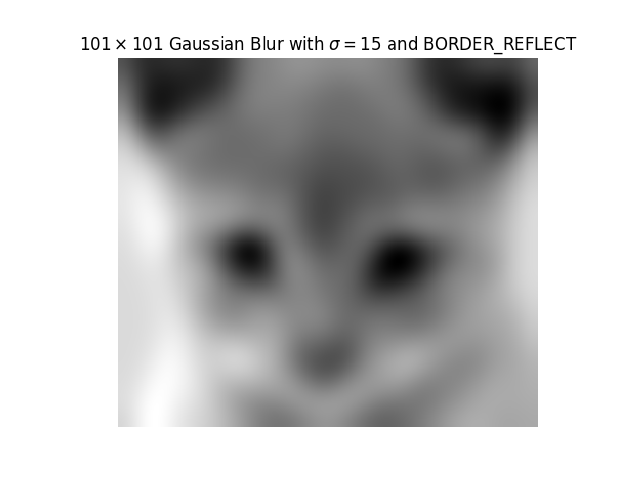
\includegraphics[scale=0.47]{img/gauss-border1.png}
	\subcaption{Borde reflejando la imágen.}
	\label{fig:gauss-border1}
\end{subfigure}
\begin{subfigure}{.5\textwidth}
	\centering
	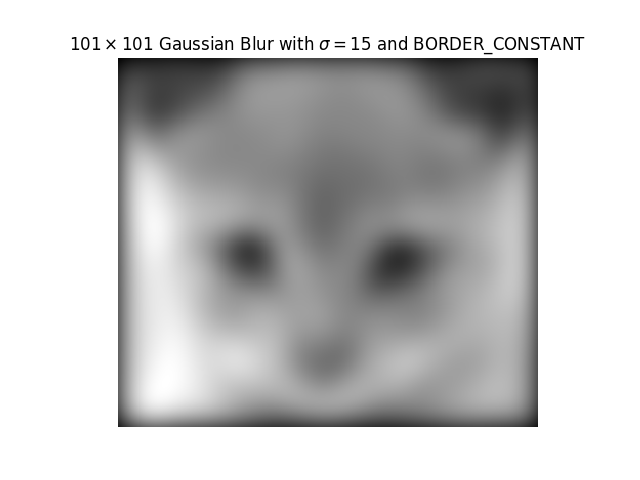
\includegraphics[scale=0.47]{img/gauss-border2.png}
	\subcaption{Borde constante.}
	\label{fig:gauss-border2}
\end{subfigure}
\end{figure}
\begin{figure}[H]\ContinuedFloat
\begin{subfigure}{\textwidth}
	\centering
	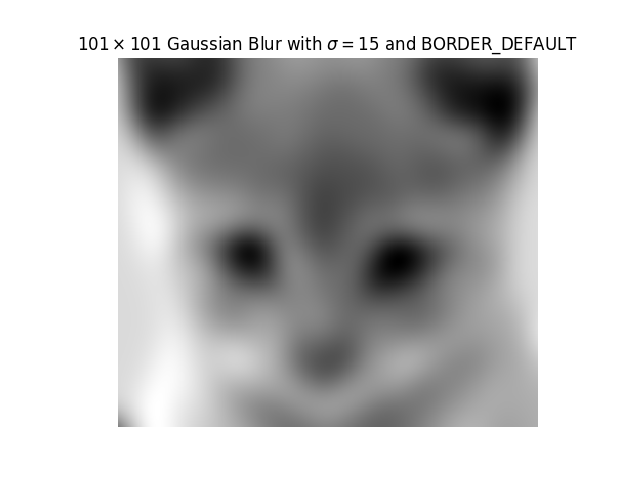
\includegraphics[scale=0.5]{img/gauss-border3.png}
	\subcaption{Borde por defecto (reflejado sin contar el primer píxel).}
	\label{fig:gauss-border3}
\end{subfigure}
\caption{Filtro Gaussiano con diferentes tipos de bordes.}
\label{fig:gauss-borders}
\end{figure}

Como se puede ver, existen ciertas diferencias dependiendo de qué tipo de borde se escoja. Si comparamos las figuras
\ref{fig:gauss-border1} y \ref{fig:gauss-border3} con la figura \ref{fig:gauss-border2}, se puede ver claramente que
los resultados no son los mismos, ya que en este último caso se utiliza un valor constante para las partes más allá
de los bordes de las imágenes. Por tanto, la imágen queda como si estuviese enmarcada.

Las diferencias entre las figuras \ref{fig:gauss-border1} y \ref{fig:gauss-border3} son mucho más sutiles, pero notables.
Se puede ver como por ejemplo en la figura \ref{fig:gauss-border3} la esquina inferior izquierda es más oscura, mientras
que en la figura \ref{fig:gauss-border1} es más clara. Aunque los dos tipos de borde reflejen la imágen, la forma en la
que lo hacen es distinto. $BORDER\_DEFAULT$ no considera el píxel del borde, mientras que $BORDER\_REFLECT$ sí que lo hace.
Todo esto se puede ver mejor explicado aquí. %INSERTAR REFERENCIA

Por último, y antes de pasar al \textit{kernel} de derivada, se ha probado a variar el $\sigma$ que se ha aplicado en cada
eje, manteniendo constante el tamaño del \textit{kernel}. A continuación se pueden ver cuáles han sido los rsultados obtenidos:

\begin{figure}[H]
\begin{subfigure}{.5\textwidth}
	\centering
	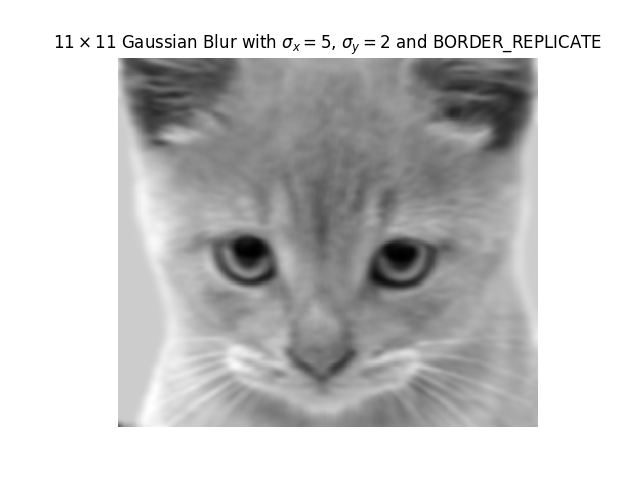
\includegraphics[scale=0.45]{img/gauss-diff1.png}
	\subcaption{Filtro Gaussiano con $\sigma_x = 5$ y $\sigma_y = 2$.}
	\label{fig:gauss-diff1}
\end{subfigure}
\begin{subfigure}{.5\textwidth}
	\centering
	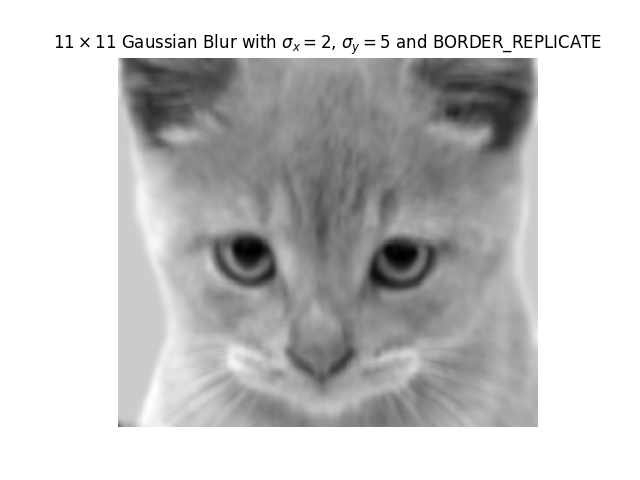
\includegraphics[scale=0.45]{img/gauss-diff2.png}
	\subcaption{Filtro Gaussiano con $\sigma_x = 2$ y $\sigma_y = 5$.}
	\label{fig:gauss-diff2}
\end{subfigure}
\caption{Filtro Gaussiano variando el $\sigma$ en cada eje.}
\label{fig:gauss-diff}
\end{figure}

Como se puede ver claramente, hay diferencias, debido a que el alisamiento solo se ha hecho en uno de los ejes en
vez de en los dos. Se puede ver como en la figura \ref{fig:gauss-diff1} el pelo de la frente del gato parece que
va hacia la derecha, mientras que en la figura \ref{fig:gauss-diff2} el pelo de la frente parece que va hacia abajo.
Además, en esta segunda imágen se puede ver como los bigotes se han emborronado más que en el primer caso, donde
son más apreciables.

Con esto ya comentado, pasemos a hablar del \textit{kernel} de las derivadas. Lo primero que podemos hacer es ver
qué influencia tiene la derivada dependiendo del eje sobre el que se aplique y según el número de veces que se derive
en cada uno de los ejes. Para ello, vamos a probar la primera y la segunda derivada en cada uno de los ejes de forma
separada (esto es, que no derivaremos a la vez). A continuación se pueden ver los resultados:

\begin{figure}[H]
\begin{subfigure}{.5\textwidth}
	\centering
	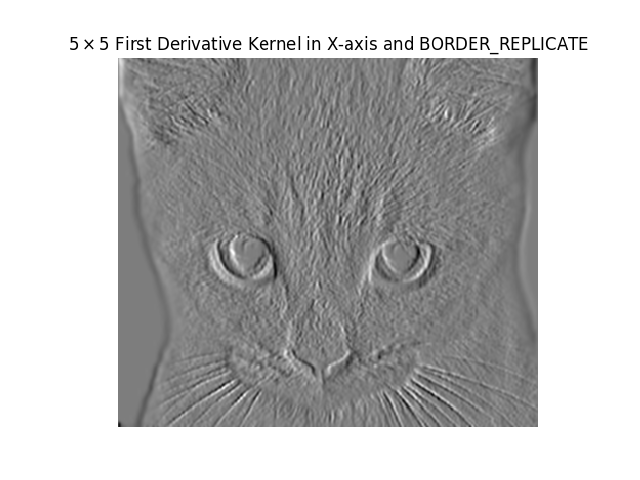
\includegraphics[scale=0.45]{img/der-x1.png}
	\subcaption{Filtro de primera derivada en el eje $X$.}
	\label{fig:der-x1}
\end{subfigure}
\begin{subfigure}{.5\textwidth}
	\centering
	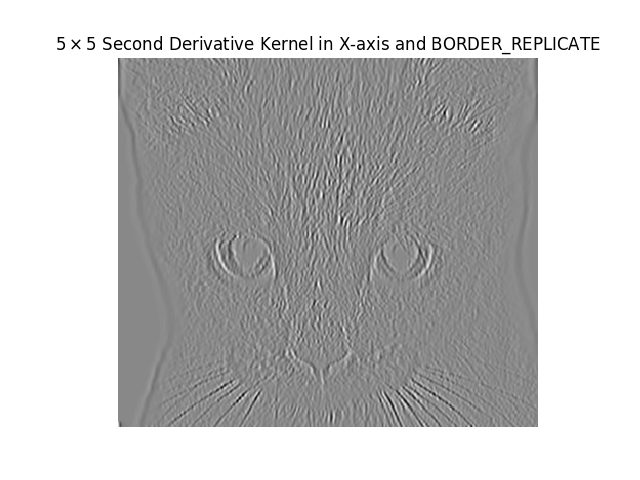
\includegraphics[scale=0.45]{img/der-x2.png}
	\subcaption{Filtro de segunda derivada en el eje $X$.}
	\label{fig:der-x2}
\end{subfigure}
\end{figure}
\begin{figure}[H]\ContinuedFloat
\begin{subfigure}{.5\textwidth}
	\centering
	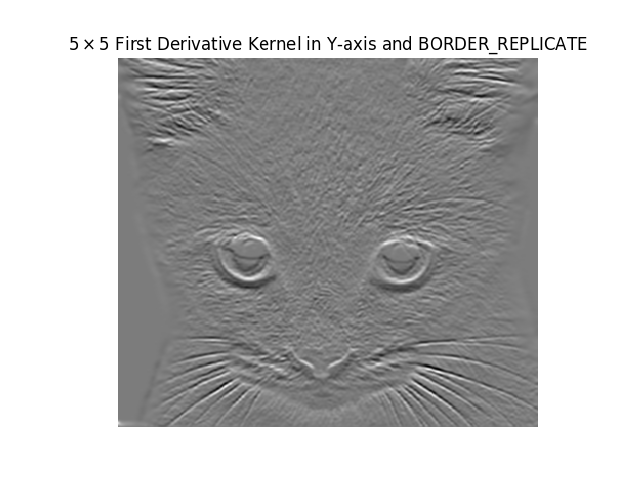
\includegraphics[scale=0.45]{img/der-y1.png}
	\subcaption{Filtro de primera derivada en el eje $Y$.}
	\label{fig:der-y1}
\end{subfigure}
\begin{subfigure}{.5\textwidth}
	\centering
	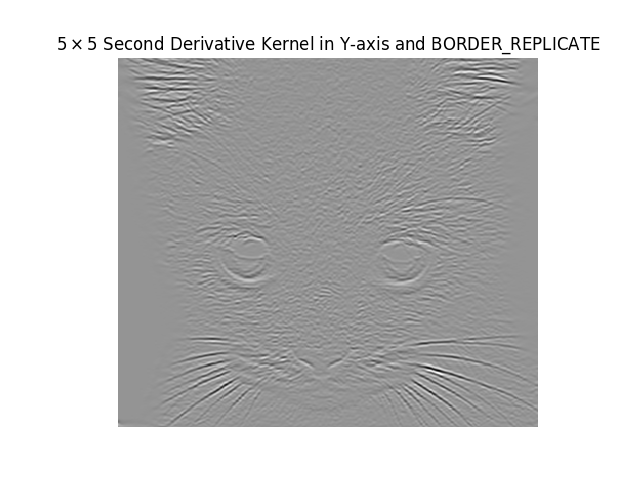
\includegraphics[scale=0.45]{img/der-y2.png}
	\subcaption{Filtro de segunda derivada en el eje $Y$.}
	\label{fig:der-y2}
\end{subfigure}
\caption{Filtro de derivada variando el número de diferenciaciones en cada eje.}
\label{fig:der}
\end{figure}

Al pasarlo por el eje $X$, como se puede ver en las figuras \ref{fig:der-x1} y \ref{fig:der-x2}, se puede ver que se van
quedando aquellos bordes verticales, ya que los horizontales se ven muy poco o nada, como es por ejemplo el caso del pelo
de las orejas, el cuál casi no se ve, o algunos de los bigotes. En cambio, al pasarlo por el eje $Y$, tal y como se
puede ver en las figuras \ref{fig:der-y1} y \ref{fig:der-y2}, se van quedando aquellos bordes que horizontales.
Se puede ver que el pelo en las orejas se puede ver mejor, además de que algunos de los bigote están mejor definidos
que en el caso anterior. Lo único que se va perdiendo son los bordes del gato como tal, haciendo que, a medida que se
va derivando más en el eje $Y$, se distinga menos donde empieza el gato y donde está el fondo.

También se ha decidido estudiar qué efecto tiene pasar el \textit{kernel} de las derivadas tanto en el eje $X$ como en
el $Y$ a la vez, ya que la función $getDerivKernel$ permite especificar el número de diferenciaciones a realizar en cada
eje. Los resultados que se han obtenido son los siguientes:

\begin{figure}[H]
\begin{subfigure}{.5\textwidth}
	\centering
	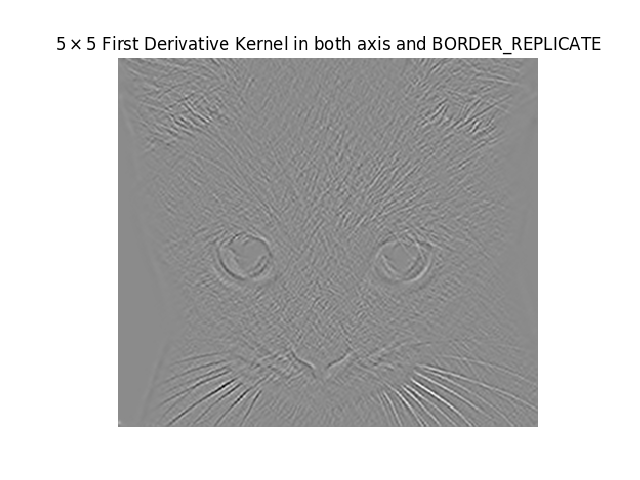
\includegraphics[scale=0.37]{img/der-xy1.png}
	\subcaption{Filtro de primera derivada en ambos ejes.}
	\label{fig:der-xy1}
\end{subfigure}
\begin{subfigure}{.5\textwidth}
	\centering
	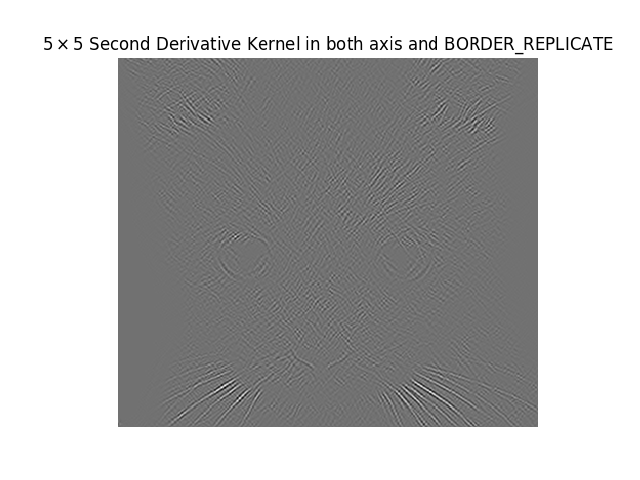
\includegraphics[scale=0.37]{img/der-xy2.png}
	\subcaption{Filtro de segunda derivada en ambos ejes.}
	\label{fig:der-xy2}
\end{subfigure}
\caption{Filtro de derivada variando el número de diferenciaciones en los dos ejes.}
\label{fig:der-xy}
\end{figure}

A diferencia de lo que se ve en la figura \ref{fig:der}, en la figura \ref{fig:der-xy} se observa que aquellos bordes que
destacan más son los que están en diagonal (es decir, una combinación de los dos ejes). Los horizontales y los verticales
casi no se notan, como por ejemplo es el caso de los contornos del gato, ya que aquí es incluso más difícil o casi imposible
distinguir donde empieza el gato y donde empieza el fondo.

Ahora, tal y como hicimos antes, pasemos a ver qué pasa si mantenemos el número de diferenciaciones constante y aumentamos
el tamaño del \textit{kernel}. Para ello, vamos a establecer que en todos los casos se obtiene la primera derivada en el eje
$X$. Los resultados de estas variaciones del tamaño del \textit{kernel} se pueden ver a continuación:

\begin{figure}[H]
\begin{subfigure}{.5\textwidth}
	\centering
	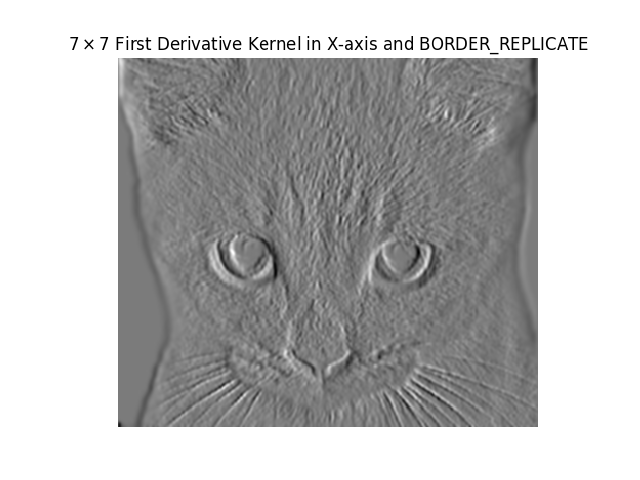
\includegraphics[scale=0.46]{img/der-size1.png}
	\subcaption{Filtro de tamaño $7 \times 7$.}
	\label{fig:der-size1}
\end{subfigure}
\begin{subfigure}{.5\textwidth}
	\centering
	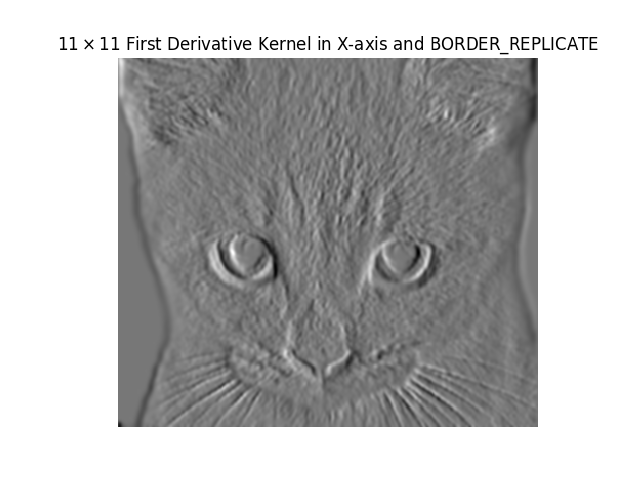
\includegraphics[scale=0.46]{img/der-size2.png}
	\subcaption{Filtro de tamaño $11 \times 11$.}
	\label{fig:der-size2}
\end{subfigure}
\begin{subfigure}{\textwidth}
	\centering
	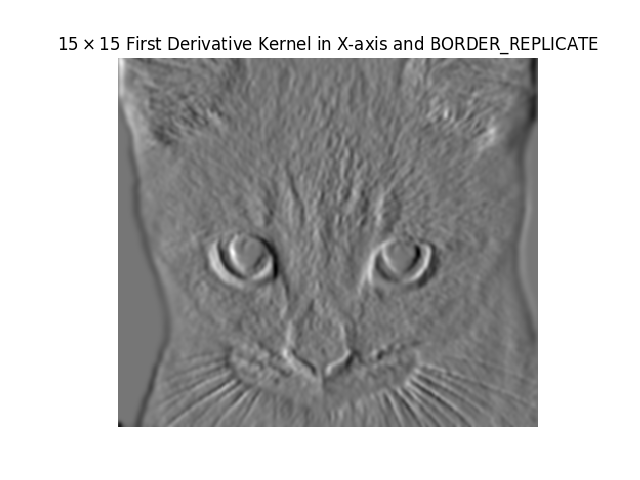
\includegraphics[scale=0.46]{img/der-size3.png}
	\subcaption{Filtro de tamaño $15 \times 15$.}
	\label{fig:der-size3}
\end{subfigure}
\caption{Filtro de primera derivada en el eje $X$ variando el tamaño del \textit{kernel}.}
\label{fig:der-size}
\end{figure}

Como resultado más obvio, se puede ver que a medida que va aumentando el tamaño del \textit{kernel}, se va emborronando más
la imágen. Esto se debe a que uno de los \textit{kernels} de Sobel hace un suavizado, de forma que se va eliminando el ruido.
A mayor tamaño del \textit{kernel}, más se va a emborronar. Por tanto, aquellos bordes muy finos se van a ir perdiendo. Por
ejemplo, si comparamos la figura \ref{fig:der-size1} con la figura \ref{fig:der-size3}, podemos ver que los bordes o contornos
que se pueden ver en la primera figura en la frente del gato han ido desapariciendo o haciéndose menos notables en esta última.
De esta forma, aumentar el tamaño del \textit{kernel} parece que solo nos aporta más suaviazado. Un tamaño de \textit{kernel}
relativamente pequeño es suficiente para extraer los contornos.

Por último, vamos a ver como variando el tipo de borde cambia la imágen que obtenemos. Para ello, tal y como hicimos antes, vamos
a fijar un tamaño de \textit{kernel} relativamente grande para poder apreciar el efecto del borde. En este caso, estamos limitados
a un tamaño máximo de 31, ya que OpenCV no permite obtener más. Por tanto, vamos a usar este tamaño de \textit{kernel} a la hora
de variar los bordes, ya que se ha considerado el más adecuado para la labor. A continuación se pueden ver los resultados:

\begin{figure}[H]
\begin{subfigure}{.5\textwidth}
	\centering
	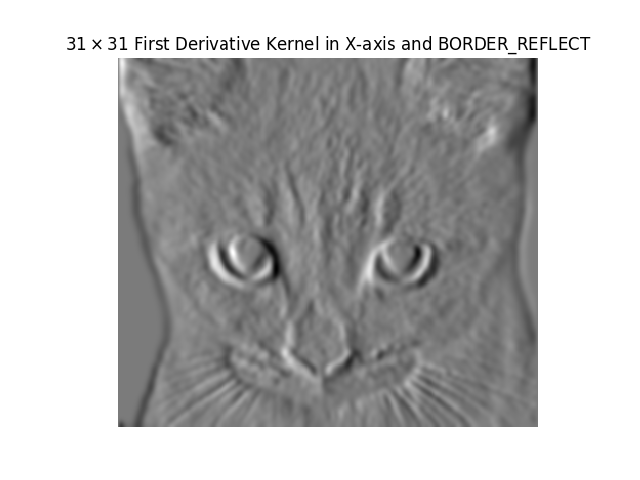
\includegraphics[scale=0.44]{img/der-border1.png}
	\subcaption{Borde reflejando la imágen.}
	\label{fig:der-border1}
\end{subfigure}
\begin{subfigure}{.5\textwidth}
	\centering
	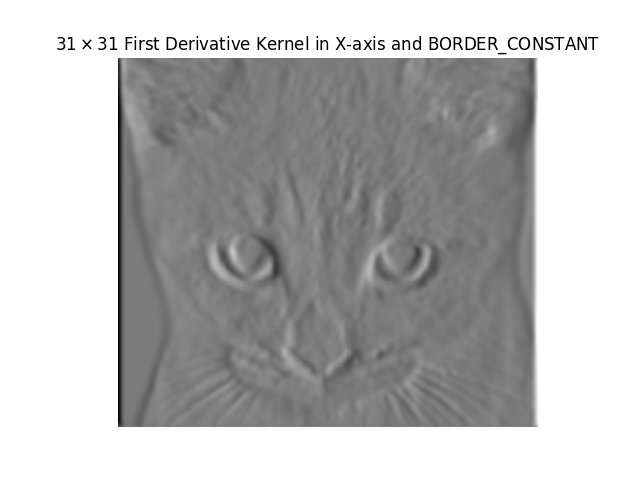
\includegraphics[scale=0.44]{img/der-border2.png}
	\subcaption{Borde constante.}
	\label{fig:der-border2}
\end{subfigure}
\begin{subfigure}{\textwidth}
	\centering
	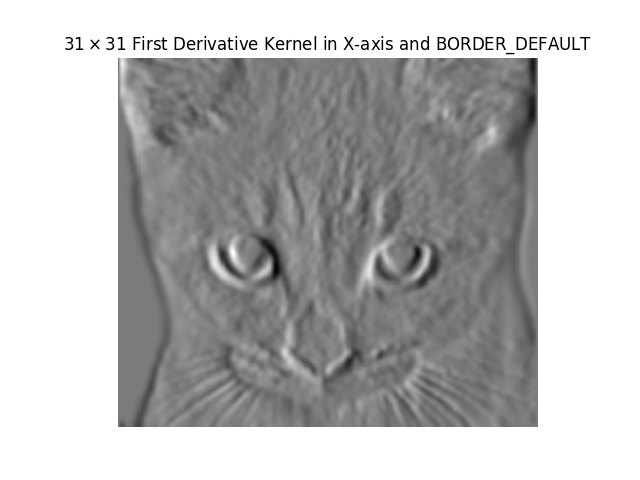
\includegraphics[scale=0.44]{img/der-border3.png}
	\subcaption{Borde por defecto (reflejado sin contar el primer píxel).}
	\label{fig:der-border3}
\end{subfigure}
\caption{Filtro de primera derivada en el eje $X$ variando el tipo de borde.}
\label{fig:der-border}
\end{figure}

En este caso, sucede algo parecido a lo que se podía ver en la figura \ref{fig:gauss-borders}. Podemos ver que
la figura más diferente de todas es la figura \ref{fig:der-border2}. Sin embargo, no parece que haya mucha diferencia
destacable o notable entre las figuras \ref{fig:der-border1} y \ref{fig:der-border3}, con lo cuál podríamos decir que
permiten obtener un resultado más o menos parecido, sin demasiadas diferencias. Parece que en este caso el tipo
de borde que más afecta es el constante, aquél en el que se supone un valor constante para todos los píxels fuera de la imágen.
Por tanto, si utilizamos cualquier otro tipo de borde no notaríamos mucha diferencia, lo cuál no sucedía en el caso del
filtro Gaussiano, ya que sí que había algunas diferencias, aunque fuesen muy pocas.

\subsection{Apartado B}

\newpage

\section{\textsc{Ejercicio sobre pirámides y detección de regiones}}

\noindent \textbf{IMPLEMENTAR} funciones para las siguiente tareas:

\begin{enumerate}[label=\textbf{\Alph*)}]
	\item \textbf{Una función que genere una representación en pirámide Gaussiana de 4 niveles de una
	imagen. Mostrar ejemplos de funcionamiento usando bordes y justificar la elección de los parámetros.}
	\item \textbf{Una función que genere una representación en pirámide Laplaciana de 4 niveles de una imagen.
	Mostrar ejemplos de funcionamiento usando bordes.}
	\item \textbf{Construir un espacio de escalas Laplaciano para implementar la búsqueda de regiones usando el siguiente
	algoritmo:}
	\begin{enumerate}[label=\textbf{\alph*.}]
		\item Fijar sigma
		\item Repetir para N escalas
		\begin{enumerate}[label=\roman*.]
			\item Filtrar la imagen con la Laplaciana-Gaussiana normalizada en escala
			\item Guardar el cuadrado de la respuesta para el actual nivel del espacio de escalas
			\item Incrementar el valor de sigma por un coeficiente k.( 1.2-1.4)
		\end{enumerate}
		\item Realizar supresión de no-máximos en cada escala
		\item Mostrar las regiones encontradas en sus correspondientes escalas. Dibujar círculos con radio proporcional a
		la escala.
	\end{enumerate}
\end{enumerate}

\subsection{Apartado A}

\subsection{Apartado B}

\subsection{Apartado C}

\newpage

\section{\textsc{Imágenes híbridas}}

\noindent \textbf{Mezclando adecuadamente una parte de las frecuencias altas de una imagen con una parte de
las frecuencias bajas de otra imagen, obtenemos una imagen híbrida que admite distintas interpretaciones a distintas
distancias (ver hybrid images project page).}

\noindent \textbf{Para seleccionar la parte de frecuencias altas y bajas que nos quedamos
de cada una de las imágenes usaremos el parámetro sigma del núcleo/máscara de alisamiento gaussiano que usaremos.
A mayor valor de sigma mayor eliminación de altas frecuencias en la imagen convolucionada. Para una buena
implementación elegir dicho valor de forma separada para cada una de las dos imágenes (ver las recomendaciones
dadas en el paper de Oliva et al.). Recordar que las máscaras 1D siempre deben tener de longitud un número impar.}

\noindent \textbf{Implementar una función que genere las imágenes de baja y alta frecuencia a partir de las
parejas de imágenes (solo en la versión de imágenes de gris). El valor de sigma más adecuado para cada pareja
habrá que encontrarlo por experimentación.}

\begin{enumerate}
	\item Escribir una función que muestre las tres imágenes (alta, baja e híbrida) en una misma ventana.
	(Recordar que las imágenes después de una convolución contienen número flotantes que pueden ser positivos y negativos)
	\item Realizar la composición con al menos 3 de las parejas de imágenes
	\item Construir pirámides gaussianas de al menos 4 níveles con las imágenes resultado. Explicar el efecto que se observa.
\end{enumerate}

\subsection{Apartado 1}

\subsection{Apartado 2}

\subsection{Apartado 3}

\newpage

\section{\textsc{Bonus}}

\subsection{Convolución 2D propia}

\noindent \textbf{Implementar con código propio la convolución 2D con cualquier máscara 2D de números reales usando
máscaras separables.}

\subsection{Imágenes híbridas a color}

\noindent \textbf{Realizar todas las parejas de imágenes híbridas en su formato a color (solo se tendrá en cuenta
si la versión de gris es correcta).}

\subsection{Imágen híbrida propia}

\noindent \textbf{Realizar una imagen híbrida con al menos una pareja de imágenes de su elección que hayan
sido extraídas de imágenes más grandes. Justifique la elección y todos los pasos que realiza.}

\newpage

\begin{thebibliography}{5}

\bibitem{nombre-referencia}
Texto referencia
\\\url{https://url.referencia.com}

\end{thebibliography}

\end{document}

